\section{Results \& Discussion}


\subsection{Signatures of \acp{IMBH} in action space}\label{results}

\begin{figure}[htbp]
\centering
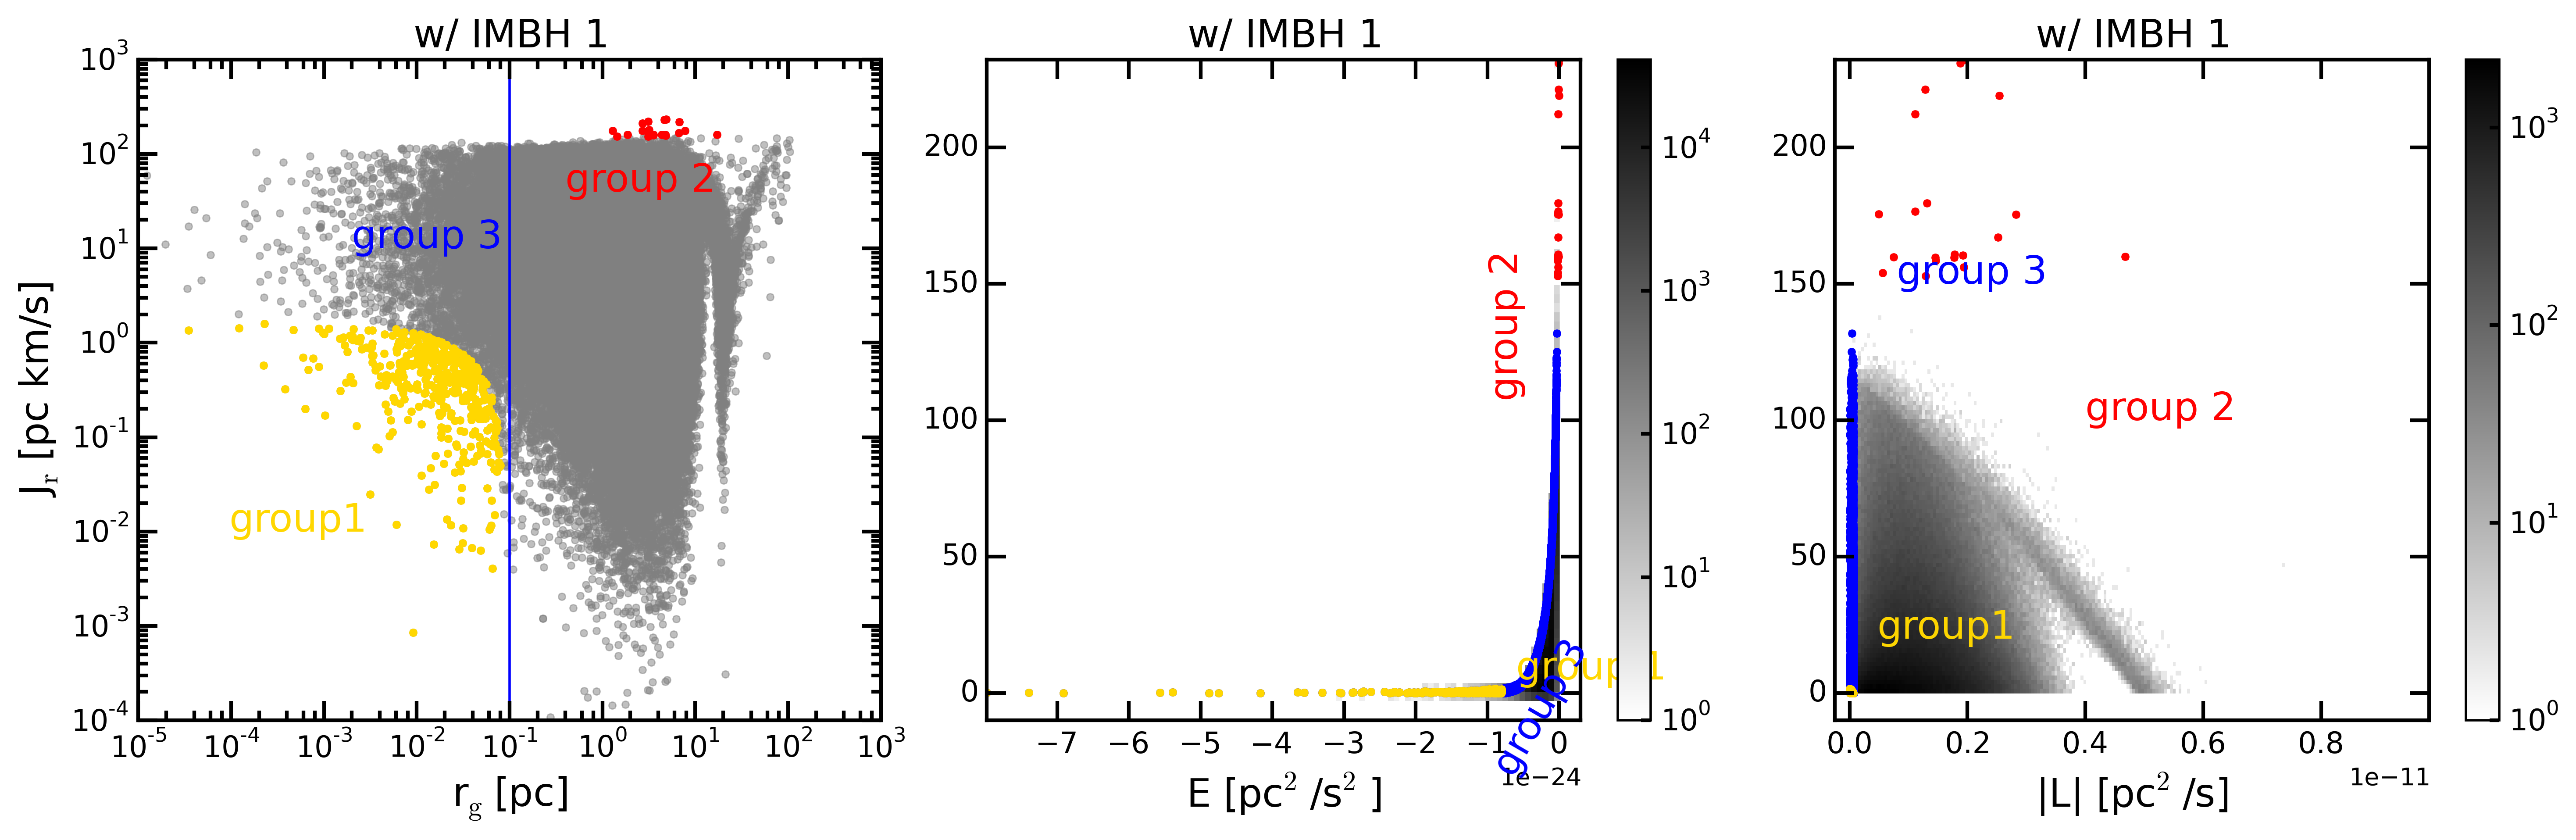
\includegraphics[width=\textwidth]{Plots/J_r_compare_plot.png}
\caption{Radial action over different values.}
\label{fig:J_r_compare}
\end{figure}

\subsection{Discussion \& future perspectives}
In summary we can say that we found clearly evidence of the \ac{IMBH} in the radial actions. To get there we made some simplified assumptions which should be investigated more precisely in an extended work. 
\par One of the assumptions regards the density profile. This is at the basis of our action approach because is is necessary to calculate the potential and from that the actions. The density is the basis of our approach of the actions. Since there is not a simple analytical function that can describe the whole profile we interpolated the binned densities and set the central density equal to the innermost density bin. Another attempt to get the density could be done by modelling Multi-Gaussian Expansion to the graph but this goes beyond the goal of our work. We test this procedure changing differnt values for the central densitieis. As a result we see that the results for section \ref{results} do not change.
\par Additional inaccuracy of the results rises due to different simulations for \acp{GC} with and without \ac{IMBH}. Since they have different initial conditions and conditions throughout the simulating process we cannot compare them directly. Especially the radial actions can not be compared since they are mass dependent. We see the differences directly in the distributions (figures \ref{fig:position_scatter} and \ref{fig:velocity_scatter}) and in the anisotropy, possibly due to different truncation prescriptions. In further investigations we should consider using simulations with same conditions despite only the absence of an \ac{IMBH} in one of the simulations. 
\par Some physical assumptions have been that actions stay totally constant over time or rather that we have only looked at them at the time of the snapshot (despite a few stars for which we integrated the orbit and have looked at the time evolution of their integrals of orbits). Changing integrals of motion go along with changing orbits which could have some numerical fluctuations especially near the \ac{IMBH}. 
\par Another assumption is that we use specific values if not said else. That means we divide all values by the mass of the stars. We see in fig \ref{fig:L_J_r_hist} that there can be distortion due to that. Further work can investigate the mass dependency of the integrals of motion. 
\par If all these points are applied to this method we should think of a way to apply this approach to observational-like data. The main difference is that at this moment there is no possibility to get the masses of the stars of \acp{GC} and therefore we can not derive the potential which is essential for this method. 




